\section{Distribuições Probabilísticas}

\subsection{Leituras Recomendadas}
\begin{frame}{Distribuições Probabilísticas - Leituras Recomendadas}
	\begin{vfilleditems}
		\item \textcite{dekkingModernIntroductionProbability2010}
		\begin{vfilleditems}
			\item Capítulo 4: Discrete random variables
			\item Capítulo 5: Continuous random variables
		\end{vfilleditems}
		\item \textcite{betancourtProbabilisticBuildingBlocks2019}
		\item \textcite{storopoli2021estatisticabayesianaR} - Distribuições Estatísticas
	\end{vfilleditems}
\end{frame}

%--- Intro -----------------------------------------------------------%
\begin{frame}{Distribuições Probabilísticas}
	A estatística Bayesiana usa distribuições probabilísticas como o motor de sua inferência na elaboração dos
	valores dos parâmetros estimados e suas incertezas.
	\vfill
	Imagine que distribuição probabilísticas são pequenas peças de "Lego". Podemos construir o que quisermos com
	essas pequenas peças. Podemos fazer um castelo, uma casa, uma cidade; literalmente o que quisermos. O mesmo é
	válido para modelos probabilísticos em estatística Bayesiana. Podemos construir modelos dos mais simples aos mais
	complexo a partir de distribuições probabilísticas e suas relações entre si.
\end{frame}

\begin{frame}{Distribuições Probabilísticas}
	\begin{defn}[Função de Distribuição de Probabilidade]
		Uma função de distribuição de probabilidade é a função matemática que fornece as probabilidades de ocorrência
		de diferentes resultados possíveis para um experimento. É uma descrição matemática de um fenômeno
		aleatório em termos de seu espaço amostral e as probabilidades de eventos (subconjuntos do espaço amostral).
		$$P(X): X \to \mathbb{R} \in [0, 1]$$
		Para variáveis discretas chamamos de "massa"~
		e para variáveis contínuas chamamos de "densidade".
	\end{defn}
\end{frame}

\begin{frame}{Notação Matemática}
	Geralmente usamos a notação
	$$X \sim \text{Dist}(\theta_1, \theta_2, \dots)$$
	Onde:
	\begin{vfilleditems}
		\item $X$: variável
		\item Dist: é o nome da distribuição
		\item $\theta_1, \theta_2, \dots$: os parâmetros que definem como a distribuição se comporta.
	\end{vfilleditems}
	Toda distribuição probabilística pode ser "parameterizada"~ao especificarmos parâmetros que permitem moldarmos alguns aspectos da distribuição para algum fim específico.
\end{frame}

\begin{frame}{Função Distribuição de Probabilidade}
	\centering
	\begin{tikzpicture}
		\begin{axis}[every axis plot, line width=2pt,
				ylabel=FDP,
				xlabel={$X$},
				domain=-4:4,samples=200,
				axis x line*=bottom, % no box around the plot, only x and y axis
				axis y line*=left, % the * suppresses the arrow tips
				enlarge x limits=true, % extend the axes a bit
			]

			\addplot [blue] {gaussian(0, 1)};
		\end{axis}
	\end{tikzpicture}
\end{frame}

\begin{frame}{Distribuições Probabilísticas}
	\begin{defn}[Função de Distribuição Cumulativa]
		A função de distribuição cumulativa (\textit{cumulative distribution function} - CDF)
		de uma variável aleatória $X$ avaliada em $x$ é a probabilidade que $X$ tomará
		valores menores ou iguais à $x$:
		$$\text{CDF} = P(X \leq x)$$
	\end{defn}
\end{frame}

\begin{frame}{Função de Distribuição Cumulativa}
	\centering
	\begin{tikzpicture}
		\begin{axis}[every axis plot, line width=2pt,
				ylabel=CDF,
				xlabel={$X$},
				domain=-4:4,samples=200,
				axis x line*=bottom, % no box around the plot, only x and y axis
				axis y line*=left, % the * suppresses the arrow tips
				enlarge x limits=true, % extend the axes a bit
			]

			\addplot [blue] {normcdf(0, 1)};
		\end{axis}
	\end{tikzpicture}
\end{frame}

%--- Discrete --------------------------------------------------------%
\subsection{Distribuições Discretas}
\begin{frame}{Distribuições Discretas}
	\begin{defn}[Distribuição de Probabilidade Discreta]
		Distribuições de probabilidade discretas são aquelas que os resultados são números
		discretos: $-N, \dots, -2, 1, 0,1,2,\dots, N$ e $N \in \mathbb{Z}$. Em distribuições discretas chamamos a
		probabilidade de uma distribuição tomar certos valores como "massa". A função massa de probabilidade
		$\text{FMP}$ é a função que especifica a probabilidade da variável aleatória $X$ tomar o valor $x$:
		$$\text{FMP}(x) = P(X = x)$$
	\end{defn}
\end{frame}

\subsubsection{Uniforme Discreta}
\begin{frame}{Uniforme Discreta}
	A distribuição uniforme discreta é uma distribuição de probabilidade simétrica em que um número finito de valores
	são igualmente prováveis de serem observados. Cada um dos $n$ valores tem probabilidade igual $\frac{1}{n}$.
	\vfill
	A distribuição uniforme discreta possui dois parâmetros e sua notação é $\text{Unif}(a, b)$:
	\begin{vfilleditems}
		\item Limite Inferior ($a$)
		\item Limite Superior ($b$)
	\end{vfilleditems}
	\vfill
	Exemplo: Um dado.
\end{frame}

\begin{frame}{Uniforme Discreta}
	$$\text{Unif}(a,b) = f(x, a, b) = \frac{1}{b-a+1} \quad \text{para $a \leq x \leq b$ e $x\in \{a,a+1,\dots ,b-1,b\}$}$$
\end{frame}

\begin{frame}{Uniforme Discreta}
	\centering
	\begin{tikzpicture}
		\begin{axis}[every axis plot,
				ybar=0pt, bar width=0.3,
				ylabel=PMF,
				samples at={1,...,6}, % All plots: from 1:6, 6 samples only
				axis x line*=bottom, % no box around the plot, only x and y axis
				axis y line*=left, % the * suppresses the arrow tips
				enlarge x limits=true, % extend the axes a bit
			]

			\addplot [fill=blue] {discreteuniform(1, 6)};
			\addlegendentry{$a=1, b=6$}
		\end{axis}
	\end{tikzpicture}
\end{frame}

\subsubsection{Bernoulli}
\begin{frame}{Bernoulli}
	A distribuição de Bernoulli descreve um evento binário de um sucesso de um experimento.
	Geralmente representamos $0$ como falha e $1$ como sucesso, então o resultado de uma distribuição de Bernoulli é
	uma variável binária $Y \in \{0, 1\}$.
	\vfill
	A distribuição de Bernoulli é muito usada para modelar resultados discretos binários no qual só há dois possíveis resultados.
	\vfill
	A distribuição de Bernoulli possui apenas um único paramêtro e sua notação é $\text{Bernoulli} (p)$:
	\begin{vfilleditems}
		\item Probabilidade de Sucesso ($p$)
	\end{vfilleditems}
	\vfill
	Exemplo: Se o paciente sobreviveu ou morreu ou se o cliente conclui sua compra ou não.
\end{frame}

\begin{frame}{Bernoulli}
	$$\text{Bernoulli}(p) = f(x, p)=p^{x}(1-p)^{1-x} \quad \text{para $x \in \{0,1\}$}$$ %
\end{frame}

\begin{frame}{Bernoulli}
	\centering
	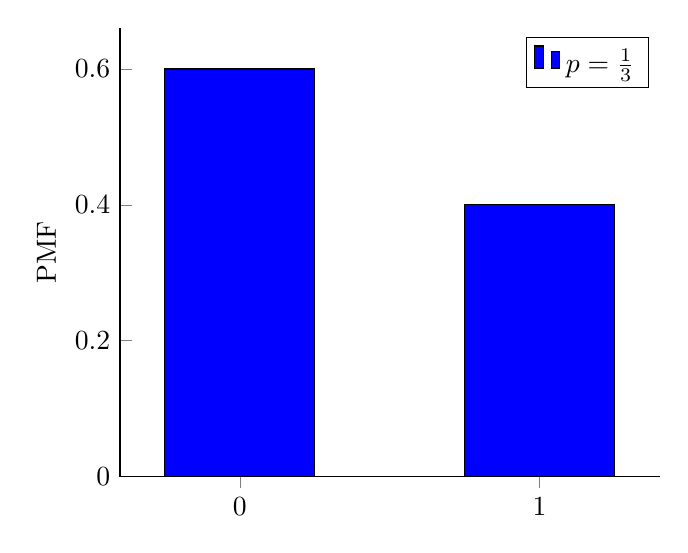
\begin{tikzpicture}
		\begin{axis}[every axis plot,
				ybar=0pt, bar width=0.5,
				ymin=0,
				xmin=-0.25, xmax=1.25,
				ylabel=PMF,
				axis x line*=bottom, % no box around the plot, only x and y axis
				axis y line*=left, % the * suppresses the arrow tips
				enlarge x limits=true, % extend the axes a bit
				xtick={0, 1}
			]

			\addplot [fill=blue] coordinates {
					(0, 0.6)
					(1, 0.4)};
			\addlegendentry{$p=\frac{1}{3}$}
		\end{axis}
	\end{tikzpicture}
\end{frame}

\subsubsection{Binomial}
\begin{frame}{Binomial}
	A distribuição binomial descreve um evento do número de sucessos em uma sequência de $n$ experimentos independentes,
	cada um fazendo uma pergunta sim-não com probabilidade de sucesso $p$. Note que a distribuição de Bernoulli é
	um caso especial da distribuição binomial no qual o número de experimentos é $1$.
	\vfill
	A distribuição binomial possui dois parâmetros e sua notação é $\text{Bin}(n, p)$ ou $\text{Binomial}(n, p)$:
	\begin{vfilleditems}
		\item Número de Experimentos ($n$)
		\item Probabilidade de Sucessos ($p$)
	\end{vfilleditems}
	\vfill
	Exemplo: quantidade de caras em 5 lançamentos de uma moeda.
\end{frame}

\begin{frame}{Binomial}
	$$\text{Binomial}(n,p) = f(x, n, p) = \binom{n}{x}p^{x}(1-p)^{n-x} \quad \text{para $x \in \{0, 1, \dots, n\}$}$$
\end{frame}

\begin{frame}{Binomial}
	\centering
	\begin{tikzpicture}
		\begin{axis}[every axis plot,
				ybar=0pt, bar width=1,
				ylabel=PMF,
				ytick={0,0.05,...,0.15},
				samples at={0,...,40},
				axis x line*=bottom, % no box around the plot, only x and y axis
				axis y line*=left, % the * suppresses the arrow tips
				enlarge x limits=true, % extend the axes a bit
				y tick label style={/pgf/number format/.cd, fixed, fixed zerofill, precision=2}
			]

			\addplot [fill=blue, fill opacity=0.5] {binomial(40, 0.2)};
			\addlegendentry{$n=40, p=\frac{1}{5}$}
			\addplot [fill=red, fill opacity=0.5] {binomial(40, 0.5)};
			\addlegendentry{$n=40, p=\frac{1}{2}$}
		\end{axis}
	\end{tikzpicture}
\end{frame}

\subsubsection{Poisson}
\begin{frame}{Poisson}
	A distribuição Poisson expressa a probabilidade de um determinado número de
	eventos ocorrerem em um intervalo fixo de tempo ou espaço se esses eventos
	ocorrerem com uma taxa média constante conhecida e independentemente do tempo
	desde o último evento. A distribuição de Poisson também pode ser usada
	para o número de eventos em outros intervalos especificados, como distância,
	área ou volume.
	\vfill
	A distribuição Poisson possui um parâmetro e sua notação é $\text{Poisson}(\lambda)$:
	\begin{vfilleditems}
		\item Taxa ($\lambda$)
	\end{vfilleditems}
	\vfill
	Exemplo: Quantidade de e-mails que você recebe diariamente. Quantidade de buracos que você encontra na rua.
\end{frame}

\begin{frame}{Poisson}
	$$\text{Poisson}(\lambda) = f(x, \lambda) = \frac{\lambda^x e^{-\lambda}}{x!} \quad \text{para $\lambda > 0$}$$
\end{frame}

\begin{frame}{Poisson}
	\centering
	\begin{tikzpicture}
		\begin{axis}[every axis plot,
				ybar=0pt, bar width=1,
				ylabel=PMF,
				samples at={0,...,8},
				axis x line*=bottom, % no box around the plot, only x and y axis
				axis y line*=left, % the * suppresses the arrow tips
				enlarge x limits=true, % extend the axes a bit
			]

			\addplot [fill=blue, fill opacity=0.5] {poisson(1)};
			\addlegendentry{$\lambda=2$}
			\addplot [fill=red, fill opacity=0.5] {poisson(4)};
			\addlegendentry{$\lambda=4$}
		\end{axis}
	\end{tikzpicture}
\end{frame}

\subsubsection{Binomial Negativa}
\begin{frame}{Binomial Negativa\footnote{Qualquer fenômeno que pode ser modelo com uma distribuição de Poisson, pode ser modelo com uma distribuição binomial negativa \parencite{gelman2013bayesian, gelman2020regression}.}}
	\small
	A distribuição binomial negativa descreve um evento do número de sucessos em uma
	sequência de $n$ experimentos independentes, cada um fazendo uma pergunta sim-não
	com probabilidade $p$ até que se obtenha $k$ sucessos. Note que ela se torna
	idêntica à distribuição de Poisson quando no limite de $k \to \infty$. Isto faz
	com que seja uma opção robusta para substituir uma distribuição de Poisson para
	modelar fenômenos com uma \textit{superdispersão} (variação nos dados excedente ao
	esperado).
	\vfill \small
	A distribuição negativa binomial possui dois parâmetros e sua notação é
	$\text{Binomial Negativa}(k, p)$:
	\begin{vfilleditems}
		\small
		\item Número de Sucessos ($k$)
		\item Probabilidade de Sucessos ($p$)
	\end{vfilleditems}
	\vfil \small
	Exemplo: Contagem anual de ciclones tropicais.
\end{frame}

\begin{frame}{Binomial Negativa}
	$$
		\begin{aligned}
			\text{Binomial Negativa}(k, p) & = f(x, k, p) & = \binom{x + k - 1}{k - 1}p^{x}(1-p)^{k} \\
			\\
			                               & ~            & \text{para $x \in \{0, 1, \dots, n\}$}
		\end{aligned}
	$$
\end{frame}

\begin{frame}{Binomial Negativa}
	\centering
	\begin{tikzpicture}
		\begin{axis}[every axis plot,
				ybar=0pt, bar width=1,
				ylabel=PMF,
				samples at={0,...,8},
				axis x line*=bottom, % no box around the plot, only x and y axis
				axis y line*=left, % the * suppresses the arrow tips
				enlarge x limits=true, % extend the axes a bit
			]

			\addplot [fill=blue, fill opacity=0.5] {negativebinomial(1, 0.5)};
			\addlegendentry{$k=1, p=\frac{1}{2}$}
			\addplot [fill=red, fill opacity=0.5] {negativebinomial(5,0.5)};
			\addlegendentry{$k=5, p=\frac{1}{2}$}
		\end{axis}
	\end{tikzpicture}
\end{frame}

%--- Continuous ------------------------------------------------------%

\subsection{Distribuições Contínuas}
\begin{frame}{Distribuições Contínuas}
	\begin{defn}[Distribuição de Probabilidade Contínua]
		\small
		Distribuições de probabilidade contínuas são aquelas que os resultados
		são valores em uma faixa contínua (também chamados de número reais):
		$(-\infty, +\infty) \in \mathbb{R}$.
		Em distribuições contínuas chamamos a probabilidade de uma distribuição
		tomar certos valores como "densidade". Como estamos falando sobre
		números reais não conseguimos obter a probabilidade de uma variável aleatória
		$X$ tomar o valor de $x$. Isto sempre será $0$, pois não há como especificar
		um valor exato de $x$. $x$ vive na linha dos números reais, portanto,
		precisamos especificar a probabilidade de $X$ tomar valores em um \textbf{intervalo}
		$[a,b]$. A função densidade de probabilidade $\text{FDP}$ é definida como:
		$$\text{FDP}(x) = P(a \leq X \leq b) = \int_a^b f(x) dx$$
	\end{defn}
\end{frame}

\subsubsection{Uniforme Contínua}
\begin{frame}{Uniforme Contínua}
	A distribuição uniforme contínua é uma distribuição de probabilidade simétrica em que um número infinito de intervalos de valores
	são igualmente prováveis de serem observados. Cada um dos $n$ infinitos intervalos valores tem probabilidade igual $\frac{1}{n}$.
	\vfill
	A distribuição uniforme contínua possui dois parâmetros e sua notação é $\text{Unif}(a, b)$:
	\begin{vfilleditems}
		\item Limite Inferior ($a$)
		\item Limite Superior ($b$)
	\end{vfilleditems}
\end{frame}

\begin{frame}{Uniforme Contínua}
	$$\text{Unif}(a,b) = f(x, a, b) = \frac{1}{b-a} \quad \text{para $a \leq x \leq b$ e $x \in [a, b]$}$$
\end{frame}

\begin{frame}{Uniforme Contínua}
	\centering
	\begin{tikzpicture}
		\begin{axis}[every axis plot, line width=2pt,
				ylabel=PDF,
				domain=0:6,samples=200,
				axis x line*=bottom, % no box around the plot, only x and y axis
				axis y line*=left, % the * suppresses the arrow tips
				enlarge x limits=true, % extend the axes a bit
			]

			\addplot [blue] {continuousuniform(0, 6)};
			\addlegendentry{$a=0, b=6$}
		\end{axis}
	\end{tikzpicture}
\end{frame}

\subsubsection{Normal}
\begin{frame}{Normal}
	Essa distribuição geralmente é usada nas ciências sociais e naturais para
	representar variáveis contínuas na qual as suas distribuições não são conhecidas.
	Esse pressuposto é por conta do teorema do limite central. O teorema do limite
	central afirma que, em algumas condições, a média de muitas amostras (observações)
	de uma variável aleatória com média e variância finitas é ela própria uma variável
	aleatória cuja distribuição converge para uma distribuição normal à medida que o
	número de amostras aumenta.
	\vfill
	Portanto, as quantidades físicas que se espera sejam a
	soma de muitos processos independentes (como erros de medição) muitas vezes têm
	distribuições que são quase normais.
\end{frame}

\begin{frame}{Normal}
	A distribuição normal possui dois parâmetros e sua notação é
	$\text{Normal}(\mu, \sigma^2)$ ou $\text{N}(\mu, \sigma^2)$:
	\begin{vfilleditems}
		\item Média ($\mu$): média da distribuição e também a moda e a mediana
		\item Desvio Padrão ($\sigma$) (às vezes também parametrizada com a variância $\sigma^2$): é uma medida de dispersão das observações em relação à média
	\end{vfilleditems}
	\vfill
	Exemplo: Altura, Peso etc.
\end{frame}

\begin{frame}{Normal\footnote{veja como a distribuição Normal foi derivada a partir da distribuição binomial nos \hyperlink{appendixnormal}{Slides de Backup no final dessa apresentação}}}
	$$\text{Normal}(\mu,\sigma) = f(x, \mu, \sigma) = \frac{1}{\sigma{\sqrt{2\pi }}}e^{-{\frac{1}{2}}\left({\frac {x-\mu }{\sigma }}\right)^{2}} \quad \text{para $\sigma > 0$}$$
\end{frame}

\begin{frame}{Normal}
	\centering
	\begin{tikzpicture}
		\begin{axis}[every axis plot, line width=2pt,
				ylabel=PDF,
				domain=-4:6,samples=200,
				axis x line*=bottom, % no box around the plot, only x and y axis
				axis y line*=left, % the * suppresses the arrow tips
				enlarge x limits=true, % extend the axes a bit
			]

			\addplot [blue] {gaussian(0, 1)};
			\addlegendentry{$\mu=0, \sigma=1$}
			\addplot [red] {gaussian(0, 2)};
			\addlegendentry{$\mu=0, \sigma=2$}
			\addplot [yellow] {gaussian(2, 1)};
			\addlegendentry{$\mu=2, \sigma=1$}
		\end{axis}
	\end{tikzpicture}
\end{frame}

\subsubsection{Log-Normal}
\begin{frame}{Log-Normal}
	A distribuição Log-normal é uma distribuição de probabilidade contínua de uma
	variável aleatória cujo logaritmo é normalmente distribuído. Assim, se a variável
	aleatória $X$ for distribuída normalmente por $\log$ natural ($\ln$),
	então $Y = \ln(X)$ terá uma distribuição normal.
	\vfill
	Uma variável aleatória com distribuição logarítmica aceita apenas valores reais
	positivos. É um modelo conveniente e útil para medições em ciências exatas e de
	engenharia, bem como medicina, economia e outros campos, por ex. para energias,
	concentrações, comprimentos, retornos financeiros e outros valores.
	\vfill
	Um processo log-normal é a realização estatística do produto multiplicativo de
	muitas variáveis aleatórias independentes, cada uma das quais positiva.
\end{frame}

\begin{frame}{Log-Normal}
	A distribuição log-normal possui dois parâmetros e sua notação é
	$\text{Log-Normal}(\mu, \sigma^2)$:
	\begin{vfilleditems}
		\item Média ($\mu$): média do logaritmo natural ($\ln$) da distribuição
		\item Desvio Padrão ($\sigma$): a variância do logaritmo natural da distribuição ($\sigma^2$) é uma medida de dispersão das observações em relação à média
	\end{vfilleditems}
\end{frame}

\begin{frame}{Log-Normal}
	$$\text{Log-Normal}(\mu,\sigma) = f(x, \mu, \sigma) = \frac{1}{x \sigma{\sqrt{2\pi}}}e^{-\left({\frac {(\ln(x)-\mu)^2}{2 \sigma^2 }}\right)} \quad \text{para $\sigma > 0$}$$
\end{frame}

\begin{frame}{Log-Normal}
	\centering
	\begin{tikzpicture}
		\begin{axis}[every axis plot, line width=2pt,
				ylabel=PDF,
				domain=0:5,samples=200,
				axis x line*=bottom, % no box around the plot, only x and y axis
				axis y line*=left, % the * suppresses the arrow tips
				enlarge x limits=true, % extend the axes a bit
			]

			\addplot [blue] {lognormal(0, 0.25)};
			\addlegendentry{$\mu=0, \sigma=\frac{1}{4}$}
			\addplot [red] {lognormal(0, 1)};
			\addlegendentry{$\mu=0, \sigma=1$}
			\addplot [yellow] {lognormal(1, 1)};
			\addlegendentry{$\mu=1, \sigma=1$}
		\end{axis}
	\end{tikzpicture}
\end{frame}

\subsubsection{Exponencial}
\begin{frame}{Exponencial}
	A distribuição exponencial é a distribuição de probabilidade do tempo entre
	eventos que ocorrem de forma contínua e independente a uma taxa média constante.
	\vfill
	A distribuição exponencial possui um parâmetro e sua notação é
	$\text{Exp}(\lambda)$:
	\begin{vfilleditems}
		\item Taxa ($\lambda$)
	\end{vfilleditems}
	\vfill
	Exemplo: Quanto tempo até o próximo terremoto. Quanto tempo até o próximo ônibus.
\end{frame}

\begin{frame}{Exponencial}
	$$\text{Exp}(\lambda) = f(x, \lambda) = \lambda e^{-\lambda x} \quad \text{para $\lambda > 0$}$$
\end{frame}

\begin{frame}{Exponencial}
	\centering
	\begin{tikzpicture}
		\begin{axis}[every axis plot, line width=2pt,
				ylabel=PDF,
				domain=0:5,samples=200,
				axis x line*=bottom, % no box around the plot, only x and y axis
				axis y line*=left, % the * suppresses the arrow tips
				enlarge x limits=true, % extend the axes a bit
			]

			\addplot [blue] {exponential(0.5)};
			\addlegendentry{$\lambda=\frac{1}{2}$}
			\addplot [red] {exponential(1)};
			\addlegendentry{$\lambda=1$}
			\addplot [yellow] {exponential(2)};
			\addlegendentry{$\lambda=2$}
		\end{axis}
	\end{tikzpicture}
\end{frame}

\subsubsection{$t$ de Student}
\begin{frame}{$t$ de Student}
	A distribuição $t$ de Student surge ao estimar a média de uma população
	normalmente distribuída em situações onde o tamanho da amostra é pequeno e o
	desvio padrão da população é
	desconhecido\footnote{Daqui que vem o tal do teste $t$ de Student}.
	\vfill
	Se tomarmos uma amostra de $n$ observações de uma distribuição normal,
	então a distribuição $t$ com $\nu = n-1$ graus de liberdade pode ser definida
	como a distribuição da localização da média da amostra em relação à média
	verdadeira, dividida pela desvio padrão da amostra, após multiplicar
	pelo termo padronizador $\sqrt{n}$.
	\vfill
	A distribuição $t$ é simétrica e em forma de sino, como a distribuição normal,
	mas tem caudas mais longas, o que significa que é mais propensa a produzir
	valores que estão longe de sua média.
\end{frame}

\begin{frame}{$t$ de Student}
	A distribuição $t$ de Student possui um parâmetro e sua notação é
	$\text{Student}(\nu)$:
	\begin{vfilleditems}
		\item Graus de Liberdade ($\nu$): controla o quanto ela se assemelha com uma distribuição normal
	\end{vfilleditems}
	\vfill
	Exemplo: Uma base de dados cheia de outliers.
\end{frame}

\begin{frame}{$t$ de Student}
	$$\text{Student}(\nu) = f(x, \nu) = \frac{\Gamma \left(\frac{\nu+1}{2} \right)} {\sqrt{\nu\pi}\,\Gamma \left(\frac{\nu}{2} \right)} \left(1+\frac{x^2}{\nu} \right)^{-\frac{\nu+1}{2}} \quad \text{para $\nu \geq 1$}$$
\end{frame}

\begin{frame}{$t$ de Student}
	\centering
	\begin{tikzpicture}
		\begin{axis}[every axis plot, line width=2pt,
				ylabel=PDF,
				domain=-4:4,samples=200,
				axis x line*=bottom, % no box around the plot, only x and y axis
				axis y line*=left, % the * suppresses the arrow tips
				enlarge x limits=true, % extend the axes a bit
			]

			\addplot [blue] {student(1)};
			\addlegendentry{$\nu=1$}
			\addplot [red] {student(3)};
			\addlegendentry{$\nu=3$}
			\addplot [yellow] {student(30)};
			\addlegendentry{$\nu=30$}
		\end{axis}
	\end{tikzpicture}
\end{frame}

\subsubsection{Beta}
\begin{frame}{Beta}
	A distribuição beta é uma escolha natural para modelar qualquer coisa
	que seja restrita a valores entre $0$ e $1$. Portanto, é uma boa candidata
	para probabilidades e proporções.
	\vfill
	A distribuição beta possui dois parâmetros e sua notação é $\text{Beta} (\alpha, \beta)$:
	\begin{vfilleditems}
		\item Parâmetro de Forma ($\alpha$ ou às vezes $a$): controla o quanto a forma é deslocada para próximo de $1$
		\item Parâmetro de Forma ($\beta$ ou às vezes $b$): controla o quanto a forma é deslocada para próximo de $0$
	\end{vfilleditems}
	\vfill
	Exemplo: Um jogador de basquete já marcou 5 lances livres e errou 3 em um
	total de 8 tentativas - $\text{Beta}(3, 5)$
\end{frame}

\begin{frame}{Beta}
	$$\text{Beta} (\alpha, \beta) = f(x, \alpha, \beta) \frac{x^{\alpha-1}(1-x)^{\beta-1}} {\frac{\Gamma (\alpha )\Gamma (\beta )}{\Gamma (\alpha +\beta )}} \quad \text{para $\alpha,\beta > 0$ e $x \in [0, 1]$}$$
\end{frame}

\begin{frame}{Beta}
	\centering
	\begin{tikzpicture}
		\begin{axis}[every axis plot, line width=2pt,
				ylabel=PDF,
				domain=0:1,samples=200,
				axis x line*=bottom, % no box around the plot, only x and y axis
				axis y line*=left, % the * suppresses the arrow tips
				enlarge x limits=true, % extend the axes a bit
			]

			\addplot [blue] {beta(1,1)};
			\addlegendentry{$\alpha=\beta=1$}
			\addplot [red] {beta(3,2)};
			\addlegendentry{$\alpha=3,\beta=2$}
			\addplot [yellow] {beta(2,3)};
			\addlegendentry{$\alpha=2,\beta=3$}
		\end{axis}
	\end{tikzpicture}
\end{frame}
